\documentclass[addpoints,12pt]{exam}
\newcommand{\ds}{\displaystyle}
\usepackage[margin=0.8in]{geometry}
\usepackage{subcaption}
\usepackage{tikz}
\usepackage{amssymb,amsmath,graphicx,wrapfig,verbatim,wasysym, enumitem,psfragx,color}
\usepackage{multicol}


\usepackage{pgf,tikz,pgfplots}
\usepackage{stmaryrd}
\usetikzlibrary{arrows, shapes.geometric, matrix, turtle, plotmarks}




\pgfplotsset{compat=1.10}
\usepgfplotslibrary{fillbetween}
\usetikzlibrary{patterns}

\pgfdeclarelayer{background}% determine background layer
\pgfsetlayers{background,main}% order of layers

%\usepackage{fancyhdr}
%\setlength{\headheight}{13.6pt}
%\pagestyle{fancy}
%\lhead{Math 222}
%\chead{ Midterm 1 }
%\rhead{Spring 2022}

\def\FillInBlank{\rule{3truein} {.01truein}}




% Choose one option (bubbles)
\newcommand{\chooseone}{{\Large$\Circle$\ \ }}
% Choose multiple options (squares)
\newcommand{\choosemany}{{\Large$\Square$\ \ }}


\newcommand{\myleft}{\makebox[.4\textwidth]{First Name:\enspace\hrulefill}}
\newcommand{\myright}{\makebox[.4\textwidth]{Last Name:\enspace\hrulefill}}
\header{\oddeven{\myleft}{}}
    {}
    {\oddeven{\myright}{}}

\footrule

\footer{Math 211}
     {Final Exam - Fall 2024}
     {Page \thepage\ of \numpages}

\begin{document}

\begin{questions}


\newpage




\question Find each derivative. You do not need to simplify your answers.

\begin{parts}


\part[4] Find $r'(t)$ if $r(t)=\ln(t^4-2t)$

\vfill


\part[5] Find $f'(x)$ if $f(x)=\sqrt{4x^2-7x}$

\vfill


\part[5] Find $y'$ if $y=\dfrac{3}{4x^2}+\dfrac{1}{\sqrt[3]{x}}+e^6$

\vfill

\part[4] Find $g'(x)$ if $g(x)=8e^xx^3$

\vfill




\end{parts}
\newpage




\question[6] Find $f''(x)$ if $f(x)=(x^2+1)^7$. You do not need to simplify your final answer.

\newpage


\question Clearly mark the correct answer(s) for each of the following by completely filling in the
appropriate bubble. \textbf{No justification is needed.}




\begin{parts}

\part[2] \textbf{(Multiple Choice-Choose one)} Let $N(t)$ represent a country's national debt at
time $t$ years after 2010. Suppose the country finds that in 2022 ($t=12$), the national debt is
rising, but more and more slowly. Which of the following is true?

\begin{itemize}[label={}]
\item \chooseone $N'(12)$ and $N''(12)$ are both positive.
\item \chooseone $N'(12)$ and $N''(12)$ are both negative.
\item \chooseone $N'(12)$ is positive, while $N''(12)$ is negative.
\item \chooseone $N'(12)$ is negative, while $N''(12)$ is positive.
\end{itemize}


\vfill


\part[2] \textbf{(Multiple Choice-Choose one)} Let $f(x,y)=\ln(y)+\dfrac{1}{x^2+1}$. Which of the
following is the domain of $f(x,y)$?

     \vspace{0.15in}
\begin{itemize}[label={}]
\item \chooseone $\{(x,y)|\, x\neq 0, y\geq0\}$ \medskip
\item \chooseone $\{(x,y)|\,y>0\}$ \medskip
\item \chooseone $\{(x,y)|\,x\neq -1, y\geq 0\}$ \medskip
\item \chooseone $\{(x,y)|\,x\neq -1, y>0\}$\medskip
\end{itemize}


\vfill




\part[2] \textbf{(True/False)} An equation for the tangent line of $f(x)=2x^2+3x$ at $x=-2$ is
$y=-5x-8$.
\begin{itemize}[label={}]
\item \chooseone True\medskip
\item \chooseone False
\end{itemize}

\vfill

\part[2] \textbf{(Multiple Choice-Choose one)} On a summer afternoon, a city's electricity
consumption is given by the rate
$E(t)$
 in units per hour, where $t$ is the number of hours after noon ($0\leq t \leq 6$).
Which of the following represents the total consumption of electricity between the hours of 1
p.m. and 4 p.m.?
\begin{itemize}[label={}]
\item \chooseone $\displaystyle \int_0^4 E(t)\; dt$ \medskip
\item \chooseone $\displaystyle \int_1^4 E(t)\; dt$ \medskip
\item \chooseone $E(4)-E(0)$\medskip
\item \chooseone $E(4)-E(1)$\medskip
\item \chooseone None of the above.
\end{itemize}

\newpage




\part[2] \textbf{(Multiple Choice-Choose one)} Suppose a study indicates that the distribution of
income for basketball players given by the Lorenz curve $L(x)=x^3$. Suppose the Gini index for
football players is $0.3$. Which profession has the more equal distribution of income?

\begin{itemize}[label={}]
\item \chooseone Basketball players \medskip
\item \chooseone Football players\medskip
\item \chooseone They are the same.
\end{itemize}

\vfill

\part[2] \textbf{(Multiple Choice-Choose one)} If $g'(x) = 4e^{2x}$ and $g(0)=5$, what is $g(x)$?
      \vspace{0.15in}
\begin{itemize}[label={}]
\item \chooseone $g(x)=2e^{2x}+3$\medskip
\item \chooseone $g(x)=4e^{2x}+3$\medskip
\item \chooseone $g(x)=2e^{2x}+5$ \medskip
\item \chooseone $g(x)=4e^{2x}+5$ \medskip
\item \chooseone None of the above.
\end{itemize}

\vfill

\part[2] \textbf{(Multiple Choice-Choose one)} Which of the following integrals correctly
computes the shaded area between $y=x^2+1$ and $y=4-2x$ (shown below)?

\begin{minipage}{.4\textwidth}
\begin{itemize}[label={}]
\item \chooseone $\displaystyle \int_{2}^{10} (x^2-3-2x)dx $\medskip
\item \chooseone $\displaystyle \int_{-3}^1 (x^2-3-2x)dx $\medskip
\item \chooseone $\displaystyle \int_{-3}^1 (5-2x-x^2)dx $\medskip
\item \chooseone $\displaystyle \int_{-3}^1 (3-2x-x^2)dx $\medskip
\item \chooseone None of the above.
\end{itemize}
\end{minipage}
\begin{minipage}{.5\textwidth}

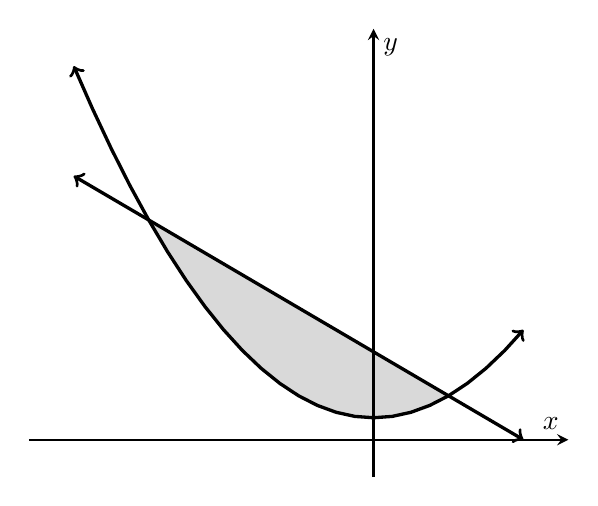
\begin{tikzpicture}[scale=1]
\begin{axis}[axis on top=true,axis lines=middle,axis line style = thick,
        xlabel=$x$,
        ylabel=$y$,
        enlargelimits,
        ytick=\empty,
        xtick=\empty
        ]

\addplot[name path=F,black, very thick,<->,domain={-4:2}] {4-2*x};

\addplot[name path=G,black,very thick,<->, domain={-4:2}] {x^2+1};


\addplot[color=gray!30]fill between[of=G and F, soft clip={domain=-3:1}];


%\node at (axis cs:2,2.45){};
\end{axis}
\end{tikzpicture}

\end{minipage}
\vfill

\end{parts}

\newpage

\question[8] Find the average value of $f(x)=6x+\dfrac{3}{4x}$ on $[2,5]$. Show all work. You do
not need to simplify your final numerical answer.

\newpage

\question[8]
A concert venue seats 200 people. When they price the tickets at $\$60$, all 200 tickets will sell.
They estimate that for each $\$3$ increase in price, they will sell 5 fewer tickets. Find the price
of concert ticket which will maximize their revenue. Justify your solution gives the maximum
revenue. Show all work.




\newpage




\question The demand function $d(x)$ and supply function $s(x)$ for a particular commodity are
given as:
$$d(x)=330-2x, \; \; s(x)=3x^2+x$$
\begin{parts}
\part[5] Find the \textbf{consumers' surplus} at demand level $A=5$. You do not need to simplify
your final numerical answer. Show all work.
\vfill
\part[5] Find the \textbf{producers' surplus} at demand level $A=5$. You do not need to simplify
your final numerical answer. Show all work.
\vfill
\part[3] Find the market demand (the positive value of $x$ at which the demand function equals
the supply function). Show all work.

\vfill
\end{parts}


\newpage

\question For $f(x,y)=6x^2-2x^3+3y^2+6xy$:

\begin{parts}
\part[5] Find $f_x, f_y, f_{xx}, f_{yy}$, and $f_{xy}$.
\vspace{3in}

\part[4] The critical points of $f(x,y)$ are $(0,0)$ and $(1,-1)$. Determine, using the $D$-test, if
each point corresponds to a relative maximum, relative minimum, or saddle point. Show all
work.

\end{parts}

\newpage

\question[8] Evaluate the following improper integral or show that it is divergent. Show all work.

$\ds \int_0^\infty \dfrac{2e^{x}+4e^{2x}}{e^{3x}}dx$

\newpage

\question For $f(x,y)=x^3-4xy-8y+3$:

\begin{parts}

\part[1] Compute $f(-1,2)$. Simplify your answer to a single number.

\vspace{1.5in}

\part[2] Find the partial derivative $f_x$.

\vspace{1.5in}

\part[2] Find the partial derivative $f_y$.

\vspace{1.5in}

\part[3] Find the critical point(s) of $f(x,y)$. Write each in the form $(x,y)$. Show all work.

\end{parts}




\newpage

\question
Use the graph of $y=f'(x)$ to answer the following. No justification is required.

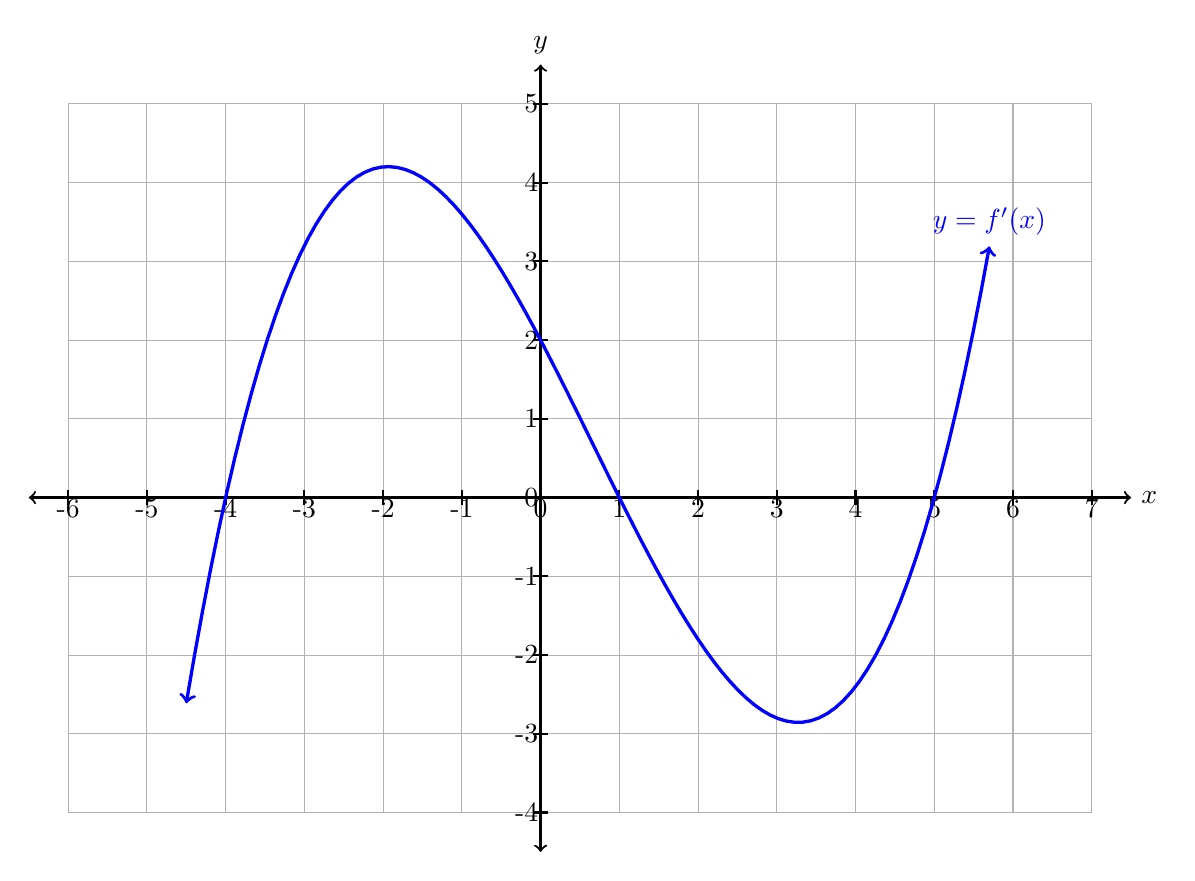
\begin{tikzpicture}[scale=1]
\draw[gray!60] (-6, -4) grid[step=1] (7, 5);

\draw[<->,thick,black] (-6.5,0)--(7.5,0) node[right]{$x$};
\draw[<->, thick,black] (0,-4.5)--(0,5.5) node[above]{$y$};
\foreach \x in {-6,-5,...,7}
\draw[thick] (\x,-.1) --(\x,.1) node[below] { \x};
\foreach \y in {-4,-3,...,5}
\draw[thick] (-.1,\y) --(.1,\y) node[left] { \y};
\draw[domain=-4.5:5.7,samples=100, very thick,<->,color=blue] plot
({\x},{(\x+4)/10*(\x-1)*(\x-5)});
\node[color=blue] at (5.7,3.5) {$y=f'(x)$};
\end{tikzpicture}

Again, \textbf{this is the graph of the derivative of $f(x)$.}

\begin{parts}
        \part[2] On which interval(s) is $f(x)$ decreasing?
 \vfill
\part[2] At which $x$-value(s) does $f(x)$ have a horizontal tangent line?
\vfill

         \part[2] What is $\displaystyle \lim_{h\to0}\frac{f(h)-f(0)}{h}$?
  \vfill
        \part[2] Is $f(x)$ concave up or concave down at $x=2$?
 \vfill




    \end{parts}




    \end{questions}

\end{document}
